\section{{\tool}: Approach Overview}
\label{overview:sec}

\begin{figure*}[t]
	\centering
	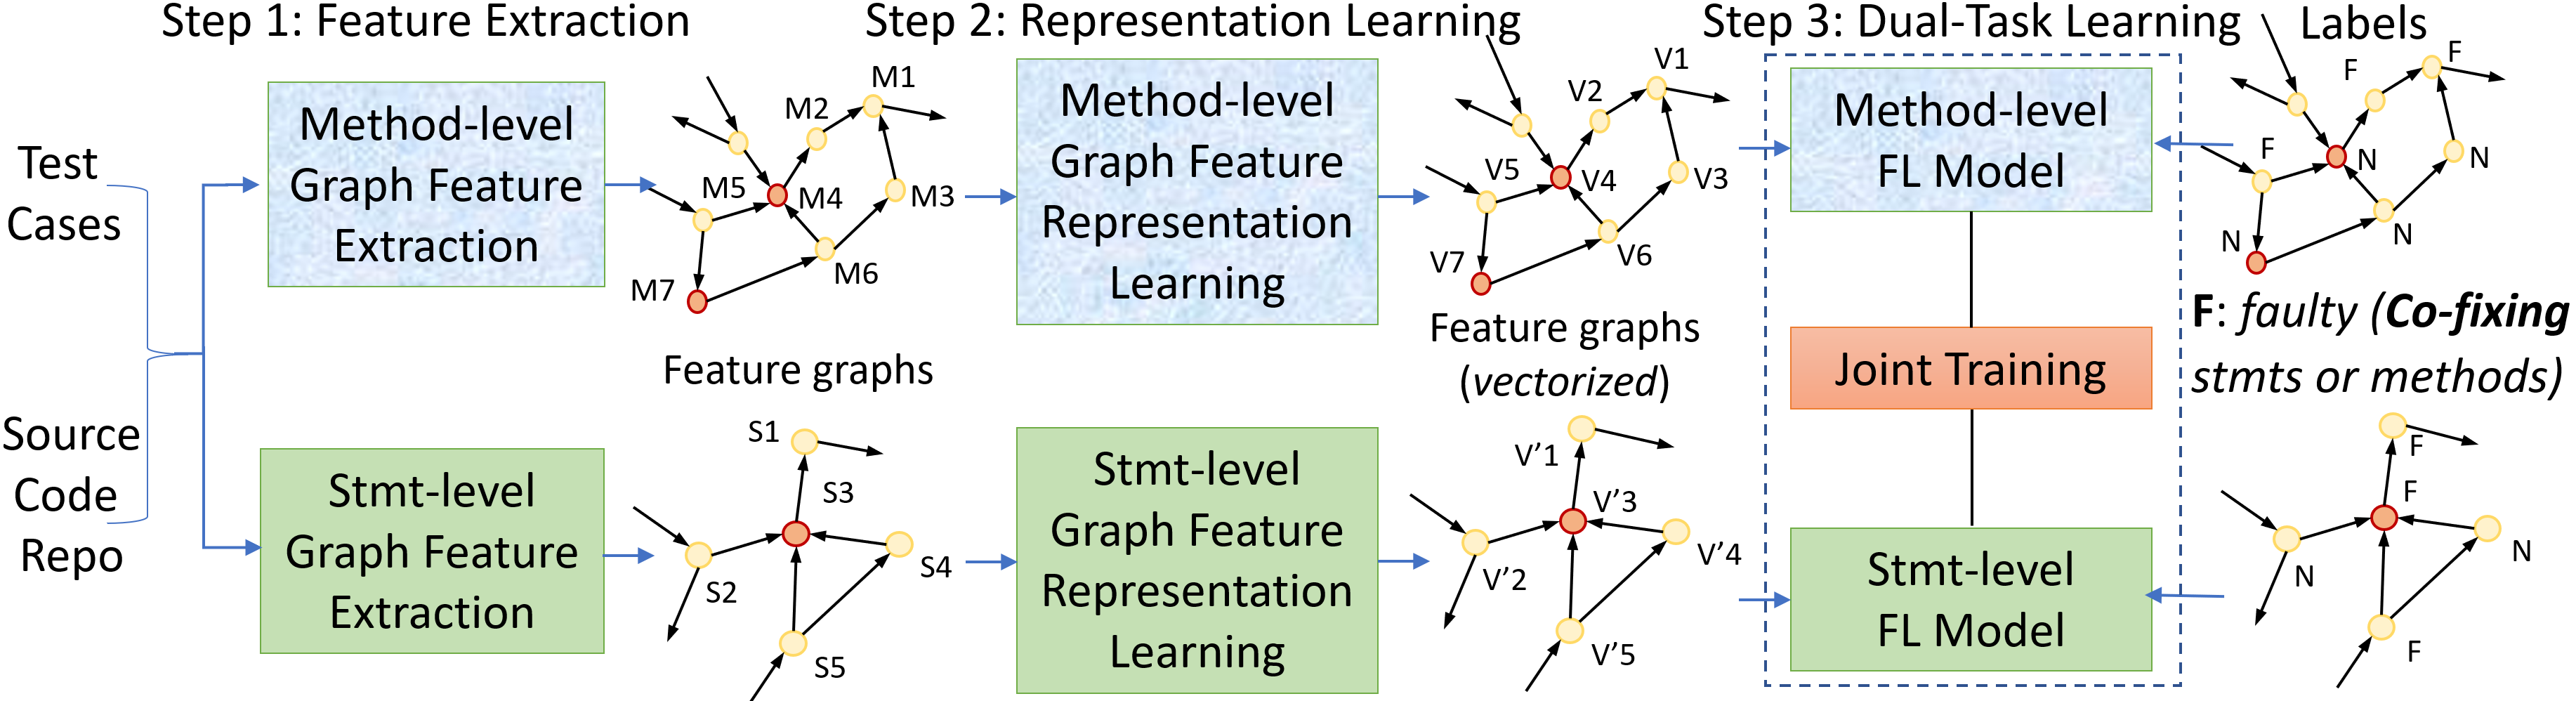
\includegraphics[width=5.65in]{graphs/overview-training-4.png} %5.45
        \vspace{-6pt}
	\caption{{\tool}: Training Process}
        \label{train-overview}
\end{figure*}

%This section presents an overview of {\tool}.

%In general, {\tool} has two processes: training and predicting.

\subsection{Training Process}


Figure~\ref{train-overview} summarizes the training process.
%
The input of training includes the passing and failing test cases, and
the source code under study.
%repository of the project under study.
The output includes the trained method-level FL model (detecting
co-fixed methods) and the trained statement-level FL model (detecting
co-fixed statements). The training process has three main~steps: 1)
{\em Feature Extraction}, 2) {\em Graph-based Feature Representation
  Learning}, and 3) {\em Dual-Task Learning Fault Localization}.

%(Figure~\ref{train-overview})

%\vspace{3pt} \noindent {\bf Step 1. Feature Extraction.}

\subsubsection{{\bf Step 1. Feature Extraction}}

(Section~\ref{feature-extract:sec}). We aim to extract the~important
features for FL from the test coverage and source code including
co-changes. The features are extracted from two levels: statements and
methods. At each level, we extract the important {\em attributes} of
statements/methods, as well as the crucial {\em relations} among
them. We use graphs to model those attributes and relations.

For \underline{a method $m$}, we collect as its attributes 1) method
content: the sequences of the sub-tokens of its code tokens (excluding
separators and special tokens), and 2) method structure: the Abstract
Syntax Tree (AST) of the method. For the relations among methods, we
extract the relations involving in the following:

1) {\em Execution flow} (the calling relation, i.e., $m$ calls $n$),

2) {\em Stack trace} after a crash, i.e., the order relation among the
methods in the stack trace (the dynamic information in execution
and stack traces have been showed to be useful in
FL~\cite{icse21-fl,DeepFL}),

3) {\em Co-change relation} in the project history (two methods that
were changed in the same commit are considered to have the co-change
relation),

4) {\em Co-fixing relation} among the methods (two methods that were
fixed for the same bug are considered to have the co-fixing relation),

5) {\em Similarity}: we also extract the similar methods in the
project that have been buggy before in the project history.
We keep only the most similar method for each method.

%(the similarity is measured on the two sequences of sub-tokens in the
%two methods).

For \underline{a statement $s$}, we extract both static and dynamic
information. First, for static data, we extract the AST subtree that
corresponds to $s$ to represent its structure. We also extract the
list of variables in $s$ together with their types, forming a sequence
of names and types, e.g., {\em ``name String price int ..."}.  Second,
for dynamic data, we encode the test coverage matrix for $s$ into the
feature vectors.
%
%In the first vector, the element corresponding to the test case $i$
%will be 1 if the test case covers $s$ and 0 otherwise. In the second
%vector, the element for the test case $i$ will be 1 if it is passing
%and 0 otherwise.

At both method and statement levels, we use graphs to represent
the methods and statements, and their relations. Let us call
them the method-level and statement-level {\em feature graphs}.




%\noindent{\bf \underline{Step 2. Graph-based Feature Representation
%    Learning.}}

%\vspace{3pt}
%\noindent{\bf Step 2. Graph-based Feature Representation Learning.}

\subsubsection{{\bf Step 2. Graph-based Feature Representation
  Learning}}

This step is aimed to learn the vector representations (i.e.,
embeddings) for the nodes in the feature graphs from step 1. The input
includes the method-level and statement-level feature graphs. The
output includes the embeddings for the nodes in the
method-/statement-level feature graphs. The graph structures for both
feature graphs are un-changed after this step.
%In this step, FixLocator aims to learn the node feature embeddings
%based on the graphs with the node features generated from step 1.
%So the input of this step is the method-level and statement-level
%graphs, and the expected output is the node embedding vectors for
%each node in each graph.

For the content of a method or statement, we use the
embedding techniques accordingly to feature representations
(Section~\ref{feature-learning:sec}). For the method's content and a
list of variables in a statement, the representation is a sequence of
sub-tokens. We use GloVe \cite{glove2014} to produce the embeddings
for all sub-tokens as we consider a method or statement as a sentence
in each case. We then use Gated Recurrent Unit (GRU)~\cite{GRU-cho14}
to produce the vector for the entire~sequence.

For the structure of a method or statement, the representation is a
(sub)tree in the AST. For this, we first use GloVe~\cite{glove2014} to
produce the embeddings for all the nodes in the sub-tree, considering
the entire method or statement as a sentence in each case. After
obtaining the sub-tree where the nodes are replaced by their GloVe's
vectors, we use TreeCaps~\cite{bui2021treecaps}, which captures well
the tree structure, to produce the embedding for the entire sub-tree.

For the code coverage representation, we directly use the two vectors
for coverage and passing/failing and concatenate them to produce the
embedding. The embedding for the most similar buggy method is computed
in the same manner as explained with GloVe and TreeCaps. Finally, the
embeddings for the attributes of the nodes are used in the fully
connected layers to produce the embedding for each node in the feature
graph at the method level. Similarly, we obtain the feature graph at
the statement level in which each node is the resulting vector of the
fully connected~layers.

%After having the six embedding vectors mentioned above, \tool uses six
%fully connected layers to standardize each embedding vector's length
%to $l/3$ (Here l/3 is an integer). And then, for both method-level and
%statement-level, \tool concatenate three feature embedding vector into
%one vector $vec_{m}$ or $vec_{s}$ for the method-level or
%statement-level with the length of $l$. In this case, for both
%method-level and statement-level, \tool all has a combined graph $G_m$
%or $G_s$ with the node embedding vector $vec_{m}$ or $vec_{s}$. It is
%the input for the next step.



%\vspace{3pt} \noindent{\bf Step 3. Dual-Task Learning Fault
%  Localization.}

\subsubsection{{\bf Step 3. Dual-Task Learning Fault
Localization}}

After the feature representation learning step, we obtain two feature
graphs at the method and statement levels, in which a node in
either graph is a vector representation. The two graphs are used as
the input for dual-task learning. For dual-task learning, we use two
Graph-based Convolution Network (GCN) models~\cite{kipf2016semi} for
the method-level FL model (\code{MethFL}) and the statement-level FL
model (\code{StmtFL}) to learn the CC fixing methods and CC fixing
statements, respectively. During training, the two feature graphs at
the method and statement levels are used as the inputs of
\code{MethFL} and \code{StmtFL}.
% Tien
%To ensure the matching of a method and its corresponding statements,
%we build the pairs ($G_M$, $g_M$) of the method-level graph $G_M$ for
%each method $M$ and the statement-level graph $g_M$ for all the
%statements in $M$. To ensure the co-fixing connections among the buggy
%methods for the same bug, in $G_M$, we model the co-fixed methods of
%$M$ via {\em co-fixed relations}. At the output layer, we label the
%nodes corresponding the faulty methods and faulty statements that were
%{\em fixed together} in the training data. A method with any faulty
%statement is labeled as faulty.
The two GCN models play the role of binary classifiers for the
bugginess for the nodes (i.e., methods/statements). We train the two
models simultaneously with soft-sharing of parameters. Details will
be given in Section~\ref{sec:dual-learning}.


%FixLocator ensures the matching of a method and its corresponding
%statements during the building of training data and the input
%processing for prediction. We build a pair (G_M, g_M) of method-level
%graph G_M and statement-level graph g_M for each method M to maintain
%that correspondence. To ensure the relations among the buggy methods
%for a bug, in G_M, we model the co-fixed methods of M via
%co-changed/fixed relations.









%as explained in Key Idea 1 in Section~\ref{sec:key-ideas}.

%We apply a probabilistic correlation as a regulization term in the
%loss function in the join training. We also design a novel constraint
%about the attention mechanism in the two models.

%For the method-level fault localization, \tool uses the GCN model
%\cite{kipf2016semi} to do the binary classification $C_m$ for each
%node based on the combined graph $G_m$. If the method is faulty, the
%GCN model will classify the node as $1$ while the GCN model classifies
%the node to $0$ when the method is non-faulty. Like the statement
%level, \tool uses the other GCN model to classify $C_s$ on the
%statement level based on the combined graph $G_s$.

%When doing the training, \tool learns the classification on both
%method-level and state-level and does the soft parameter sharing
%between the two models to make these two GCN models learn more
%features from both levels.

%\vspace{-2pt}
\subsection{Predicting Process}

\begin{figure}[t]
	\centering
	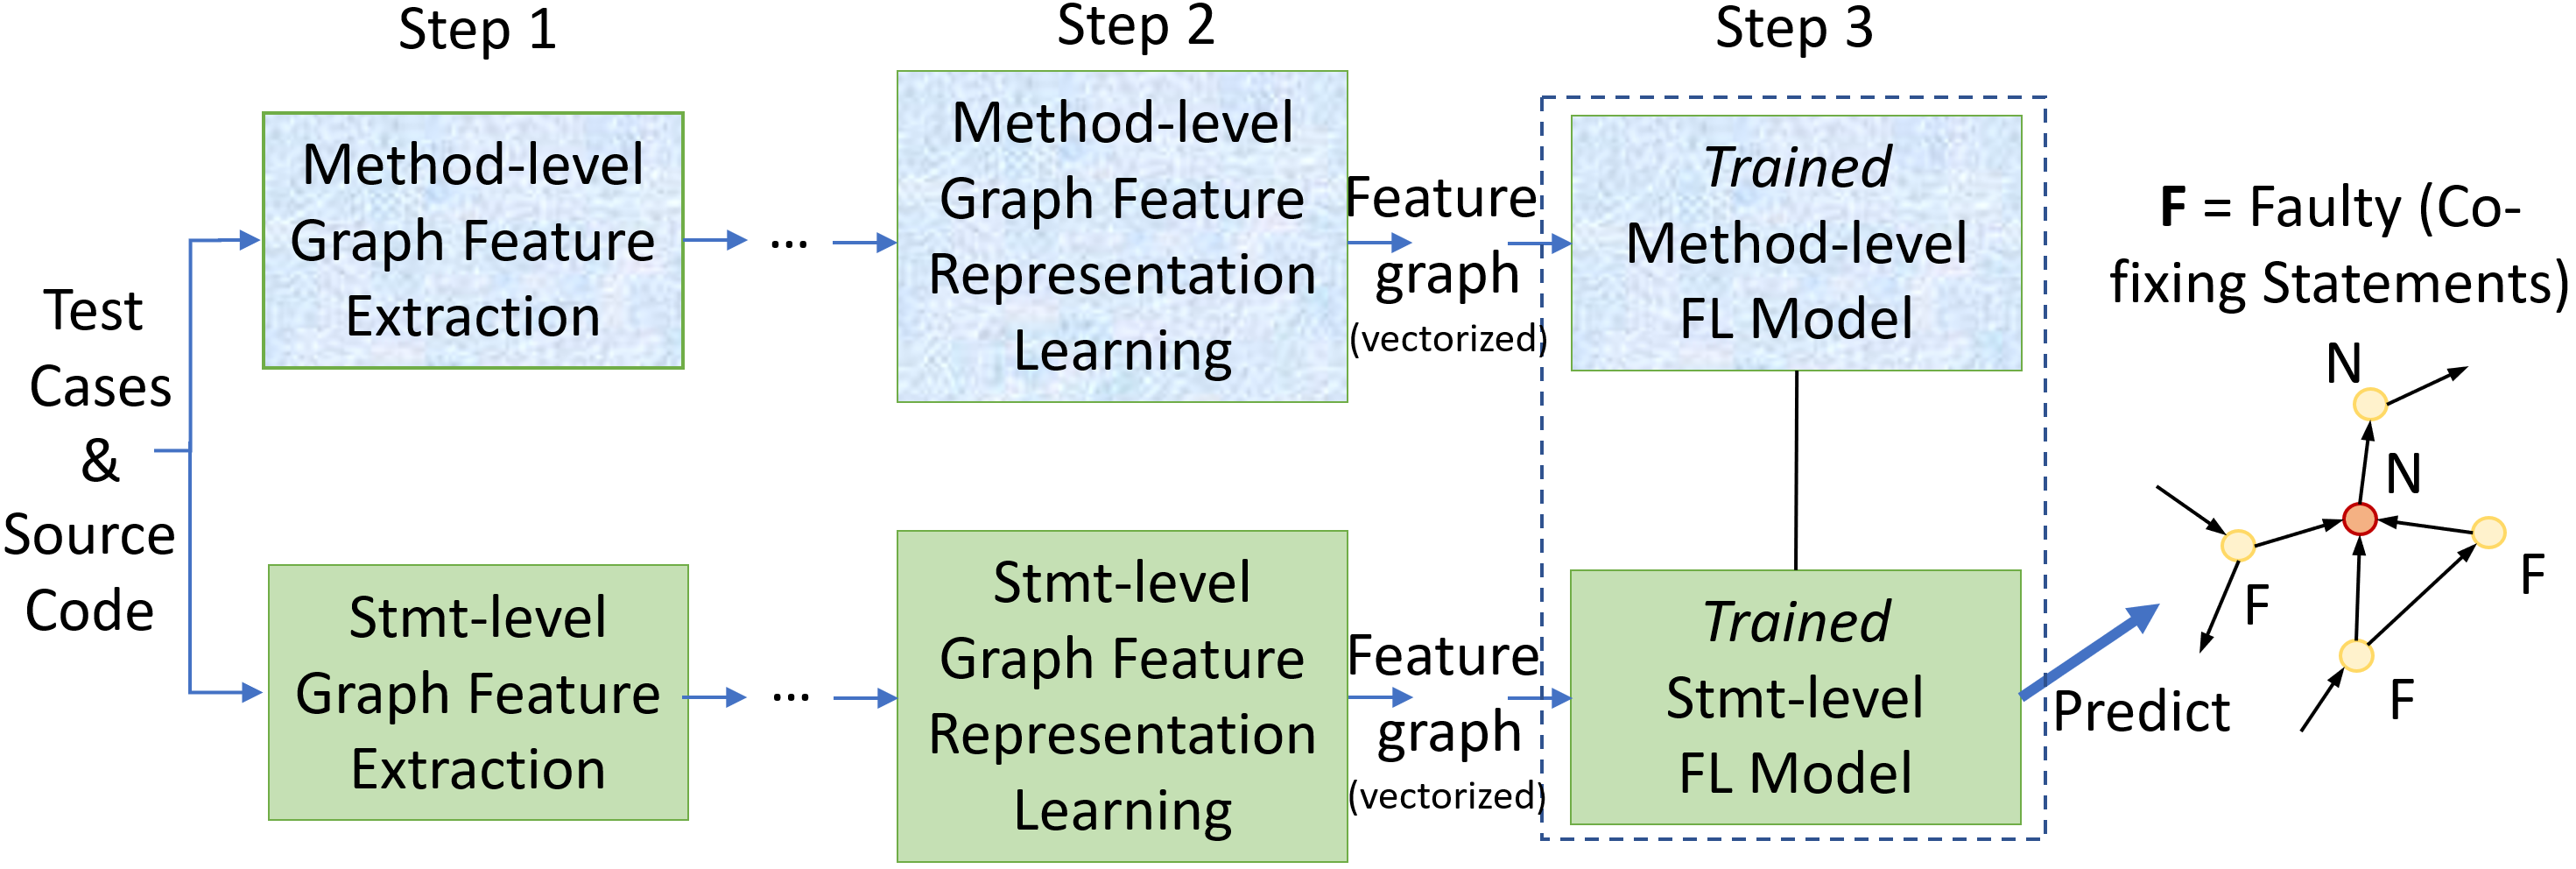
\includegraphics[width=3.3in]{graphs/overview-predict-3.png}
        \vspace{-10pt}
        \caption{{\tool}: Prediction Process}
	\label{predict-overview}
        \vspace{-6pt}
\end{figure}

The input of the prediction process (Figure~\ref{predict-overview})
includes the test cases and the source code in the project. The steps
1--2 of the process is the same as in training. In step 3, the feature
graph $g_M$ at the statement level built from the source code is
used as the input of the {\em trained} \code{StmtFL} model, which
predicts the labels of the nodes in that graph. The labels indicate
the bugginess of the corresponding statements in the source
code, which represent the CC fixing statements. If one aims to predict
the faulty methods, the trained \code{MethFL} model can be used on the
feature graph to produce the CC fixing methods.
%at the method level.

%But when making the prediction, because the statement-level fault
%localization is the primary goal, \tool only picks the statement-level
%fault localization results as the final results. Thus, \tool regards
%all the statements marked as faulty as the model output statement set,
%which contains the statements predicted to be fixed together in this
%fault.


